\chapter{Architecture}
Varroas architecture is organised as a distributed system, whereas there are two main roles in the system: the Agents and the Commander.
The Commander is the central unit that passes work packages of the Scenario to the Agents.
In contrast the Agents process the passed packages and create MQTT clients to execute the testing process.
%The Commander parses the Scenario, splits it into chunks and then distributes it among the agents.

\section{Varroa Distributed System Architecture}
\begin{figure}[h]
	\begin{center}
	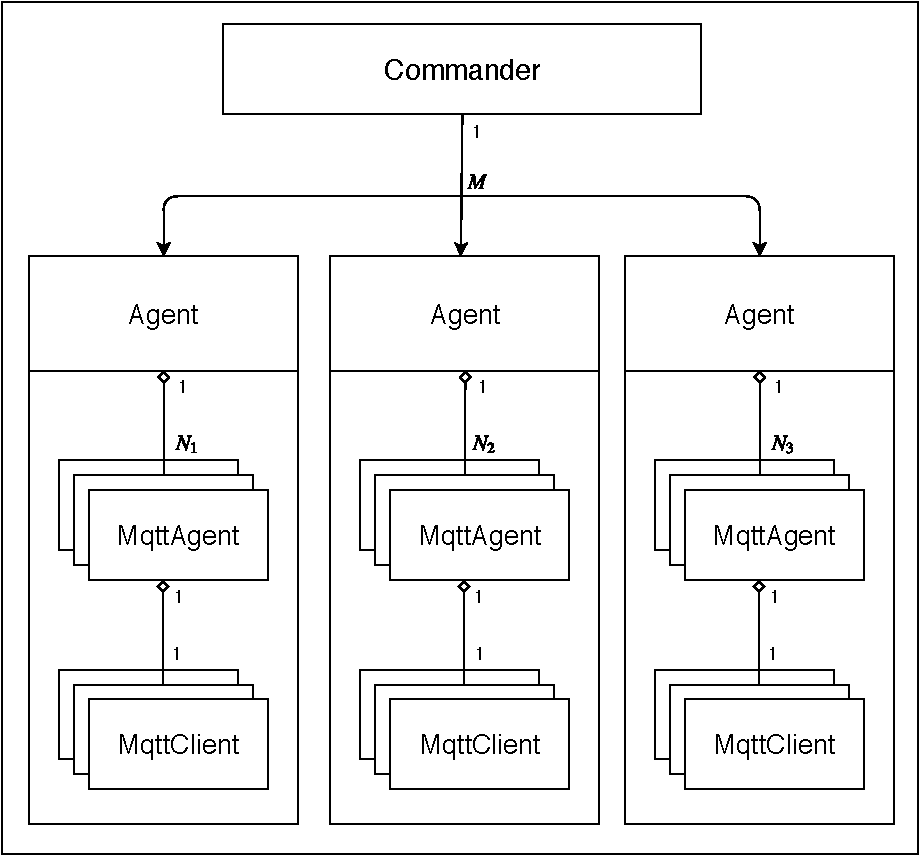
\includegraphics[scale=0.65]{Resources/PDF/Architecture}
	\caption{Varroa Distributed System Architecture}
	\label{pic:Architecture}
	\end{center}
\end{figure}
A Varroa Distributed System is composed of a Commander and multiple Agents.
The Commander and all Agents are executed in separate Varroa Instances.
Every Agent holds a number of MQTT Agents and each MQTT Agent manages one MQTT Client.
\newpage

\section{Commander}
\begin{figure}[h]
	\begin{center}
	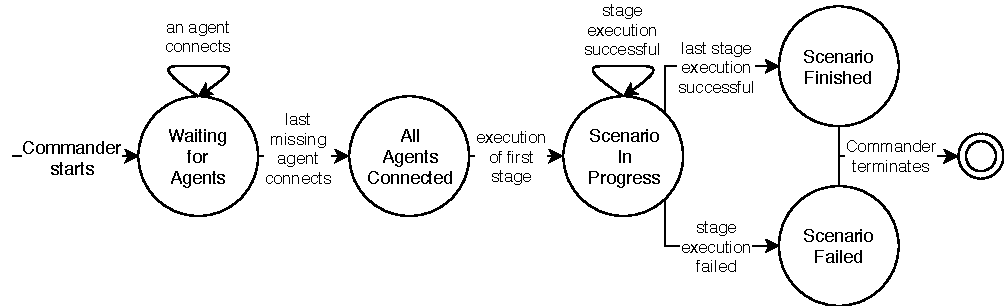
\includegraphics[scale=1]{Resources/PDF/CommanderStates}
	\caption{Commander States}
	\label{pic:CommanderStates}
	\end{center}
\end{figure}

\section{Agent}


\section{Commander Agent Communication}
\subsection{Chunk Handshake}
\begin{figure}[h]
	\begin{center}
	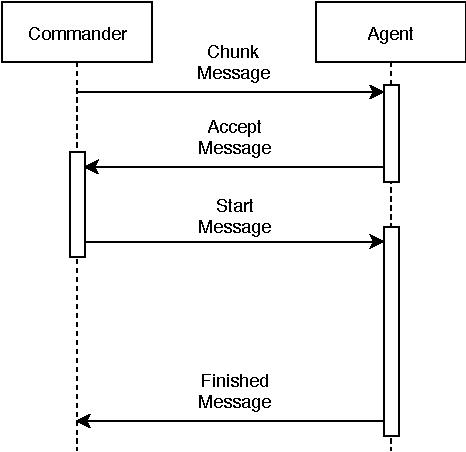
\includegraphics[scale=1]{Resources/PDF/ChunkHandshake1}
	\caption{Chunk Handshake with Accept}
	\label{pic:ChunkHandshake1}
	\end{center}
\end{figure}

\begin{figure}[h]
	\begin{center}
	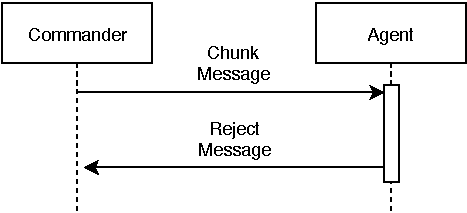
\includegraphics[scale=1]{Resources/PDF/ChunkHandshake2}
	\caption{Chunk Handshake with Reject}
	\label{pic:ChunkHandshake2}
	\end{center}
\end{figure}